S. Bre{\ss} and others benchmarked CoGaDB by using Star Schema Benchmark\cite{ssbm}, which is a popular OLAP framework frequently used for performance evalutions. By running queries provided by SSBM\footnote{Star Schema Benchmark}, CoGaDB GPU-acceleration can be compared and evaluated with the other versions such as MonetDB\footnote{Open-source column-oriented database management system}. With the help of these benchmarking, performance insights of CoGaDB can be drawn.
\begin{figure}[h]
\centering
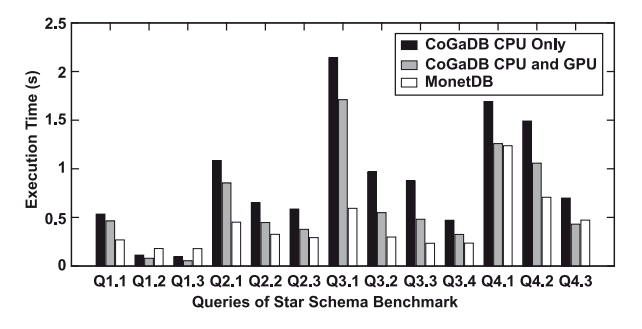
\includegraphics[width=15cm,height=15cm,keepaspectratio]{cogadb/cogadb_performance}
\caption{Response times of CoGaDB for the SSBM, taken from \cite{cogadb_design_impl}}
\label{fig:cogadbperformance}
\end{figure}
\newline 
From the Figure \ref{fig:cogadbperformance}, we can observe that CoGaDB performance is significantly improved with GPU acceleration as compared to the CPU only version. Futhermore, CoGaDB provides quite comparable and similar performance when evaluated with MonetDB. Hence, CoGaDB can be considered as a suitable GPU-accelerated platform for running heavy intensive OLAP workloads in heterogeneous processor systems.